
\documentclass{article}
\usepackage{nips13submit_e,times}

% removed below because it was for IEEE
%\documentclass[letterpaper, 10 pt, conference]{ieeeconf}  % Comment this line out if you need a4paper

% not using IEEE stuff
%\IEEEoverridecommandlockouts                              % This command is only needed if 
                                                          % you want to use the \thanks command
% remove ieee margins
%\overrideIEEEmargins                                      % Needed to meet printer requirements.


%             \documentclass{article}
%             \usepackage{nips13submit_e,times}



\usepackage{prg-stuff}

%\usepackage{ijcai09}  % style
\usepackage{times}    % font
\usepackage{graphicx} % inserting images
\usepackage{cite}
%\usepackage{amsmath}
\usepackage{mathtools} % For math
\usepackage{hyperref}
%\usepackage{enumitem}
\renewcommand{\deg}{\ensuremath{^{\circ}}\xspace}  % why doesn't this work???

\providecommand{\e}[1]{\ensuremath{\times 10^{#1}}}

\graphicspath{ {./figures/} } % Point to the figures directory

%%%%%%%%%%%%%%%%%%%%%%%%%%%%%%%%%%%%%%%%%%%%%%%%%%%%%%%%%%%%%%%%%%%%%%%%%%%

\title{\LARGE \bf 
3D Point Cloud Object Classified for ROS
}

\author{
Kory E. Kraft\\
School of Mechanical, Industrial, and Manufacturing Engineering,\\
Oregon State University\\
Corvallis, OR, 97330\\
\texttt{kraftko@onid.oregonstate.edu} \\
\And
Austin L. Nicolai\\
School of Mechanical, Industrial, and Manufacturing Engineering,\\
Oregon State University\\
Corvallis, OR, 97330\\
\texttt{nicolaia@onid.oregonstate.edu} \\
}

\newcommand{\fix}{\marginpar{FIX}}
\newcommand{\new}{\marginpar{NEW}}

\nipsfinalcopy 

\begin{document}

\maketitle
\thispagestyle{empty}
\pagestyle{empty}
\begin{abstract}
Many challenging robotics tasks require the ability to manipulate the local environment to complete a
task. Often, due to the difficulty, these tasks are accomplished using shared autonomy or teleoperation.
The need exists for robots to be able to automatically identify and manipulate the local environment on
their own. We implemented a prototype object classifier module for ROS. To test with, we classifed four common
manipulatives found in many homes.  
\end{abstract}


\section{Introduction}
Robotics is experiencing an upsurge in research, industry, and popular culture due to 
recent advances in basic robotic abilities.  Driverless vehicles are on the road, and seem to be, in more ways than 
one, right around the corner. However, even with advances in software architecture,
computing hardware, and mechanical hardware, there is still a large gap between what popular culture
 envisions robots doing and what robots can actually do today.

Similarly to computers, there exists tasks that robots can do better than humans, and tasks that humans can do
better than robots. The ideal is to have fully autonomous robots operating in the world without the need for human intervention.
There are numerous obstacles preventing that from being the current reality. In order to deploy robots in the real world as quickly as possible, to the benefit of humans, shared autonomy must be exploited to the fullest extent. Finding ways to leverage the advantages of both parties will lead to accelerations in both robot deployment and ability.

Simplifying and streamlining the robot-human interface while using what is readily available in current hardware and software will lead to a better, more fluid shared autonomy experience in less time. Robots are built to interact with the physical world at a level beyond most computer systems. To this end, they must sense the environment in order to interact with it. The Microsoft Kinect RGB-D camera is a low-cost solution for many computer vision tasks required by a robot. On the software side, the Robot Operating System (ROS), is a software system and set of libraries that currently handles basic information processing for robots in a hardware-independent manner.

What is missing between the two is a simple framework with a clean interface that unites the current hardware and software capabilities for the purposes of object classification, that will then be used for object manipulation during a shared autonomy session. To this end, we built a prototype program that utilized ROS-formatted data streams from a Microsoft Kinect along with the PyBrain machine learning package to classify four common manipulative objects: a standard light switch, a door-handle, a door-knob, and a drawer handle. These objects were classified using 3D point cloud information obtained via a Kinect sensor. Having a streamlined data to classification program will improve the current state of the art shared autonomy approach for object manipulation by removing a previously time-consuming step on the part of the human user.

\section{Related Work}
\subsection{Shared Autonomy}
In the world of robots, there is a spectrum of autonomous function.  On one end, there is a fully autonomous robot
without the need for human intervention in the direction of basic tasks.  Think, a driverless vehicles that only need to be told a destination, and then the rest is taken care of by the vehicle.  On the other end is remote teleoperation that requires a human expert to constantly inform and direct the robot.  Think, a scientist sitting a desktop using a joystick to control all the movements of a research submersible. Shared autonomy lies in the middle between these two extremes. 

Shared autonomy requires that a robot be able to do some things on its own (e.g. raise its gripper hand or drive forward), but leaves
room for a human in the loop to direct or give meaning to the robot's actions.

\begin{figure}[h!]
    \centering
    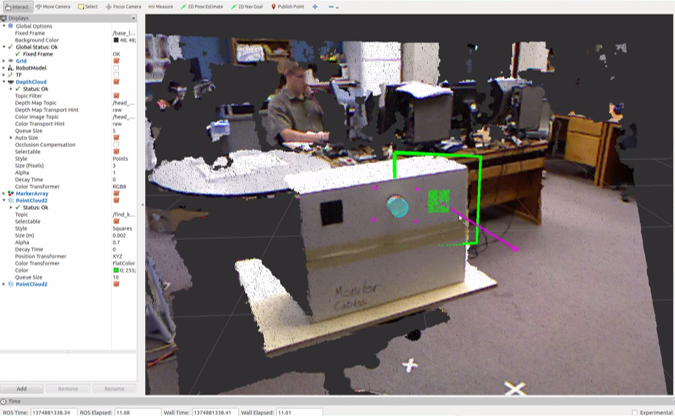
\includegraphics[width=0.45\textwidth]{Shared_Autonomy_1.png}
    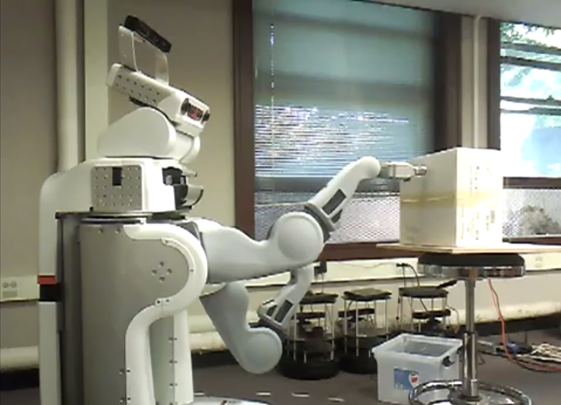
\includegraphics[width=0.45\textwidth]{Shared_Autonomy_2.png}
    \caption{...explain...}
    \label{fig:sharedAutonomy}
\end{figure}
Shared Autonomy Operation of Physical Device Controls, Matthew Rueben William D. Smart HRI LBR

\subsection{Object Classification}
Automatic classification of images and objects has long been an important task in machine learning. With the proliferation of lower cost depth capable sensors (e.g. the Microsoft Kinect), more work is being done involving the classification of point cloud and 3D image classification.

More specifically, object detection and classification using the Microsoft Kinect has been examined. [CITATION INFO] Janoch, et al. present a large 3D dataset comprised of over 50 classes after determining that current 3D datasets are lacking in scene and category variation. They further provide a method to smooth the noisy depth data provided by the Kinect, and establish baseline object detection rates. Another application by [CITATION INFO] Greuter, et al. uses Kinect point cloud data to detect game pieces (specifically, chess) and determine their board location. They were able to achieve an approximate 84\% success rate.

In the realm of personal robotics, Rusu, et al. examine the use of 3D point cloud based mapping and recognition in household environments. They present a method in which once an environment is mapped, 3D point cloud data obtained by laser scans can be mapped to the scene. The point cloud data is then segmented into regions, which are then able to be identified into kitched objects (e.g. cupboard, drawer, dishwasher, etc). Through real world testing, they were able to experimentally validate their results. [CITATION INFO NEEDED]

\subsection{ROS}
The Robot Operating System (ROS), which has some of its deepest roots in the Stanford AI group and former Willow Garage, 
has become the leader in open-source robotics software \cite{ros, rospaper}. ROS is written largely in C++ and Python and runs ontop of Ubuntu.  

It is used by hobbyists, researchers, and major industrial manufacturers, and has a large pool of active developers. The software library is vast, and due to the hardware agnostic nature of the system, ROS can run on many different robot platforms.  ROS includes tools for basic robot sensing, movement, and simulators that allow programmers to test code before deploying it on a physical robot. Although ROS is guided by Open Source Robotics Foundation (OSRF), ROS relies on the larger community to maintain and extend its capabilities \cite{ros, OSRF}.

ROS includes packages for teleoperation, using the keyboard and mouse, or even operating the robot utilizing a Razer Hydra controller and Oculus Rift headset \cite{surrogate}. ROS also includes MoveIt!, a path-planning and object manipulation software \cite{moveit}. 

Given all of the benefits of ROS, we were somewhat surprised to find that there was not a streamlined, one-step program and interface to classify objects based on 3D point cloud information that could then be used in conjunction with a shared autonomy approach and MoveIt!.

\subsection{Microsoft Kinect}
The Microsoft Kinect was introduced to the marketplace in 2010 \cite{kinectHistory}. Since then 
it has found its way into research labs as well living rooms.
It provides RGB-D sensing for less than 100 dollars. It has become a standard RGB-D
sensing device due to its low price point, extensive documentation, and large community of
adopters. The original Kinect is limited to 0.8 - 4.0m distance range and 57$^{\circ}$ horizontal 
and 43$^{\circ}$ vertical field-of-view. 

The device is not flawless; it has a random error in the depth axis 
ranging from a few mm to 4 cm in a non-uniform distribution \cite{khoshelham2012accuracy,nguyen2012modeling}.
Kinect v2 has been released that provides 3x better depth fidelity and improved small object visualization compared to 
the original Kinect \cite{kinect}. We used the original Kinect for our project that will provide a baseline for manipulative classification, which will only be improved upon for the future.

\subsection{PyBrain}
PyBrain describes itselft as ''a modular Machine Learning Library for Python.'' The open-source module focuses on neural networks and offers ways to quickly build and train neural networks, even for beginning programmers. PyBrain includes Python bindings to use other popular products like LibSvm \cite{pybrain, pybrainCode}.  

PyBrain works well alongside ROS, and depends heavily upon SciPy which is included with rospy.

\section{Methods}
\subsection{Objects}
We decided to classify four common household objects: a door knob, light switch, drawer handle, shower knob. These objects were selected
for their ubiquity in many residences and living environments. 

\begin{figure}[h!]
    \centering
    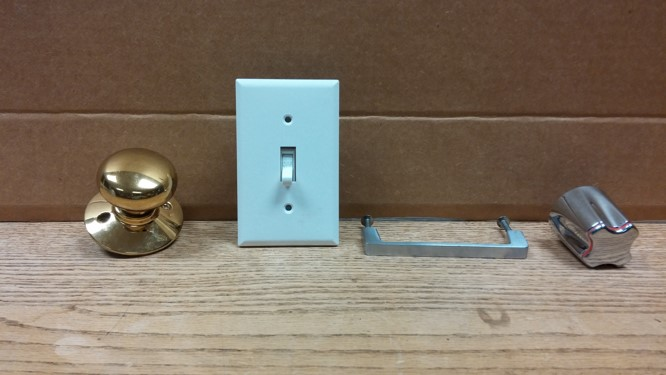
\includegraphics[width=0.45\textwidth]{All_Knobs.jpg}
    \caption{Objects Classified: door knob, light switch, drawer handle, shower knob}
    \label{fig:objects}
\end{figure}

\subsection{Data Capture}
We chose to capture the data in such a way that can be easily adapted to a near-future operation environment in which a robot will be instructed via a human trainer to ''learn'' an image that the human is pointing to.  Only capturing 5 seconds of data ensures that the capture time will be more seamless, and will not result in the human trainer waiting for enormous amounts of time for the robot to ''take in'' the scene.  

We captured data utilizing the Microsoft Kinect and subscribing to the related ROS topic.  The data was recorded into a rosbag format.  Even though we did this via a stationary laptop, we were running a virtual instance of ROS to issue the commands. This means that any robot running ROS has access to the same commands and data format. (Include figures from slide here)

For ease of operability, and to have standardized image distances during the first iteration, we decided to detach the Kinect from a robot and place it onto a tripod, with the specific object in the middle of the Kinect's field-of-view. We kept the Kinect at the same height and distance (0.8 m) while capturing the data. Approximately 5 seconds of data were captured for each manipulative (and blank backdrop) at each viewing angle. The three viewing angles, in terms of the horizontal viewing axis were: 90 degrees, and \(\pm\) 20 degrees.

The Kinect sensor provides both point cloud and RGB data at resolution of 640 x 480. For every one second of recording, approximately 10 depth registered point clouds were stored.

\subsection{Data Parsing}
We decomposed the captured image into a 640 x 480 2d color matrix and a 640 x 480 normalized 2d greyscale matrix, using values 0-255. This was done in Python utilizing ROS-pcl, a ROS interface to the open-source Point Cloud Library (PCL), and self-written code \cite{pcl, rospcl}.

\begin{figure*}
    \centering
    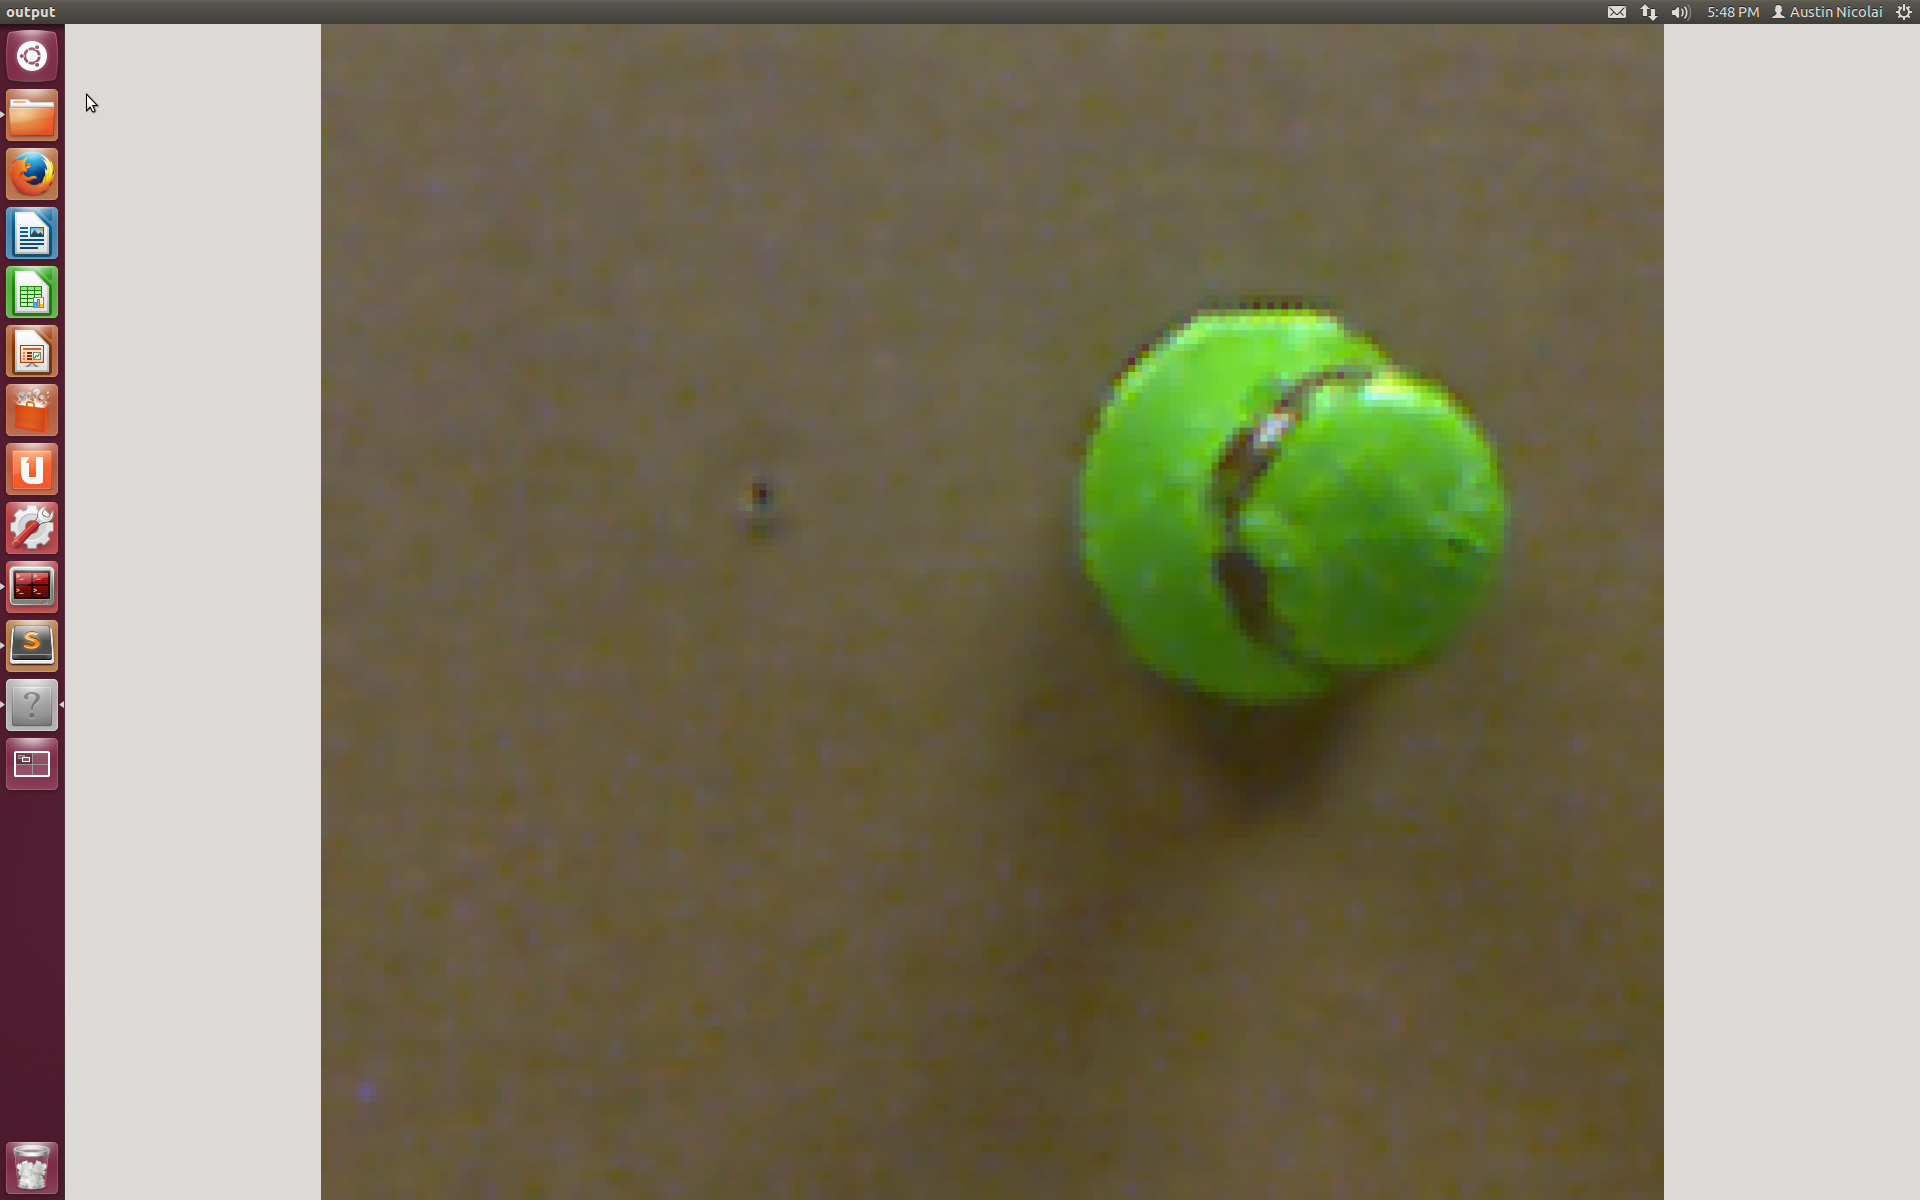
\includegraphics[width=0.3\textwidth]{DH_RGB_L.png}
    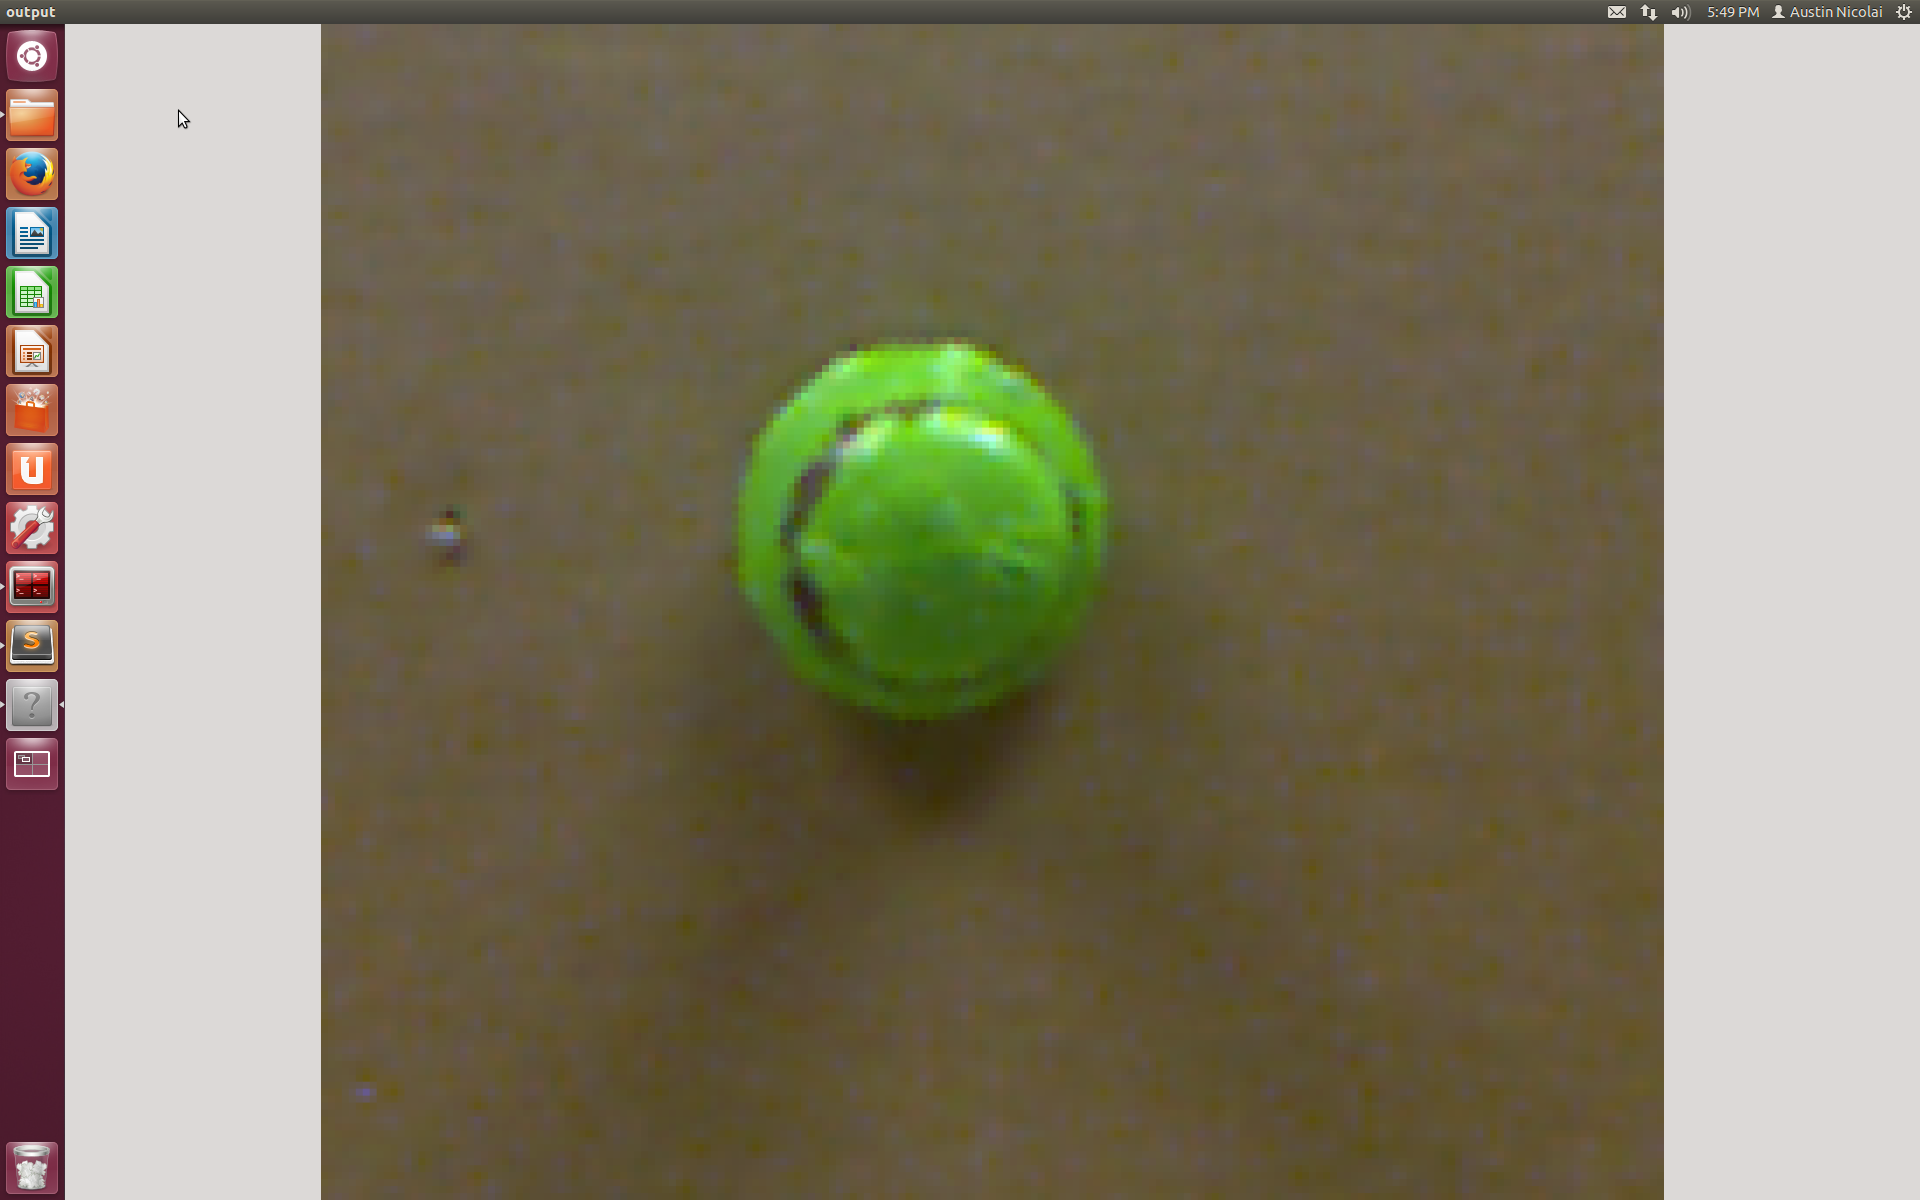
\includegraphics[width=0.3\textwidth]{DH_RGB_C.png}
    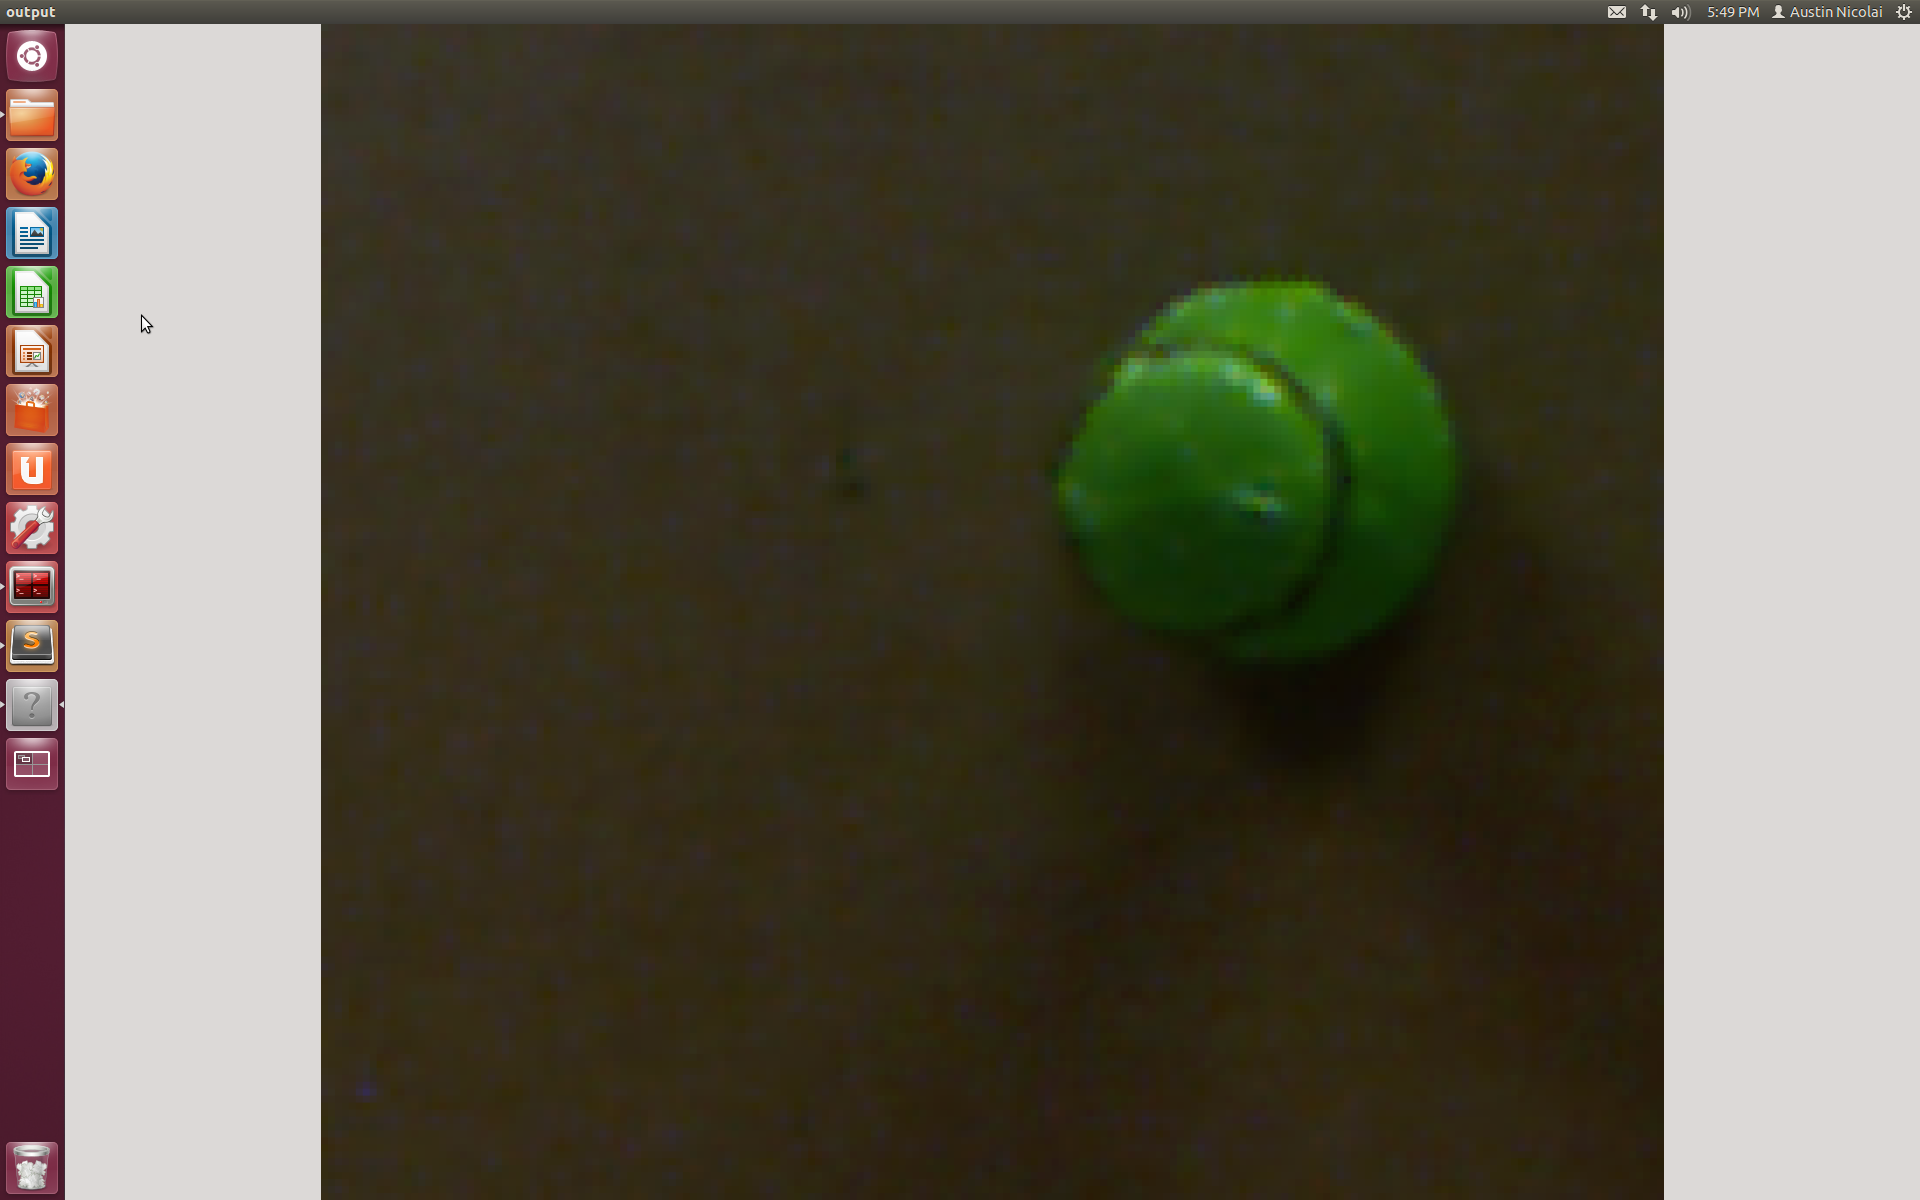
\includegraphics[width=0.3\textwidth]{DH_RGB_R.png}
    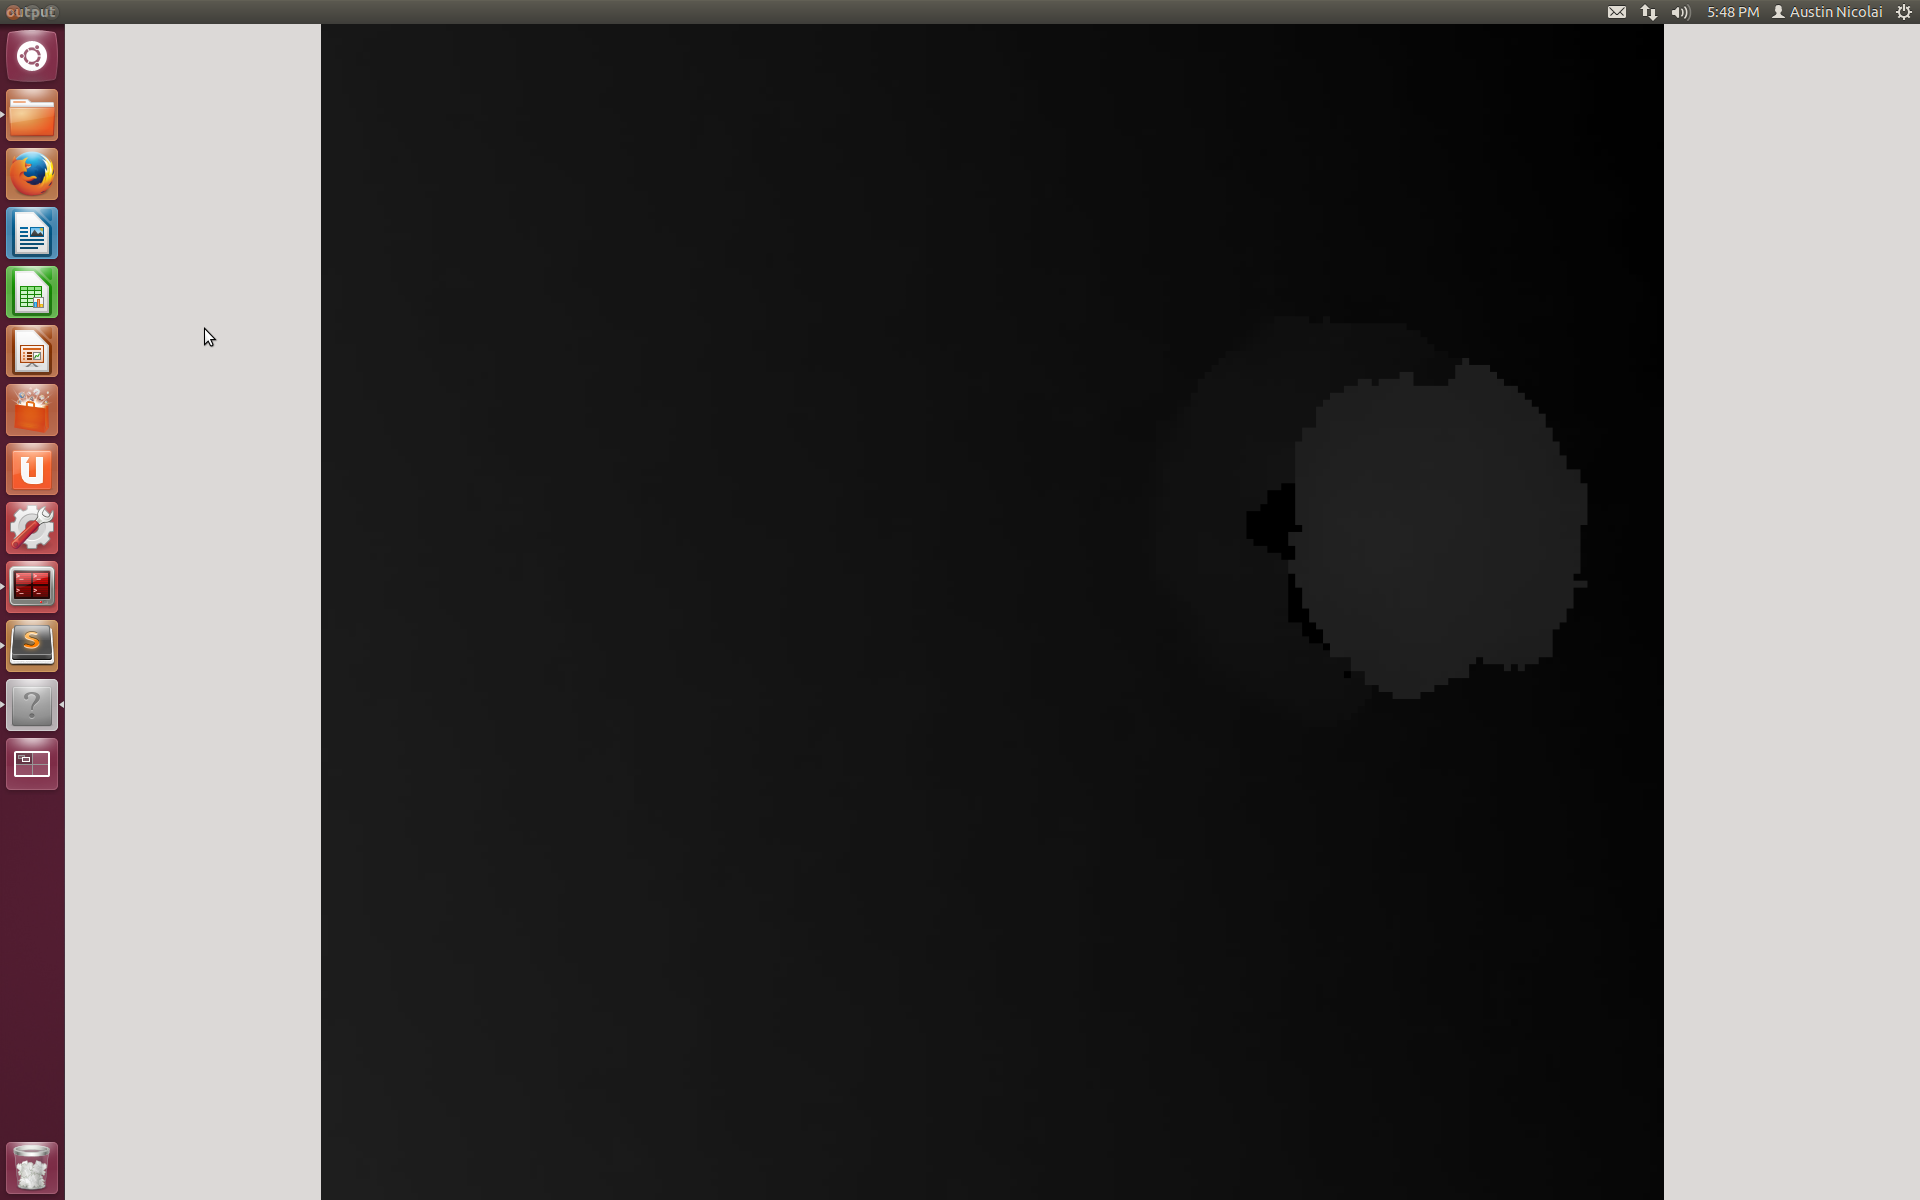
\includegraphics[width=0.3\textwidth]{DH_D_L.png}
    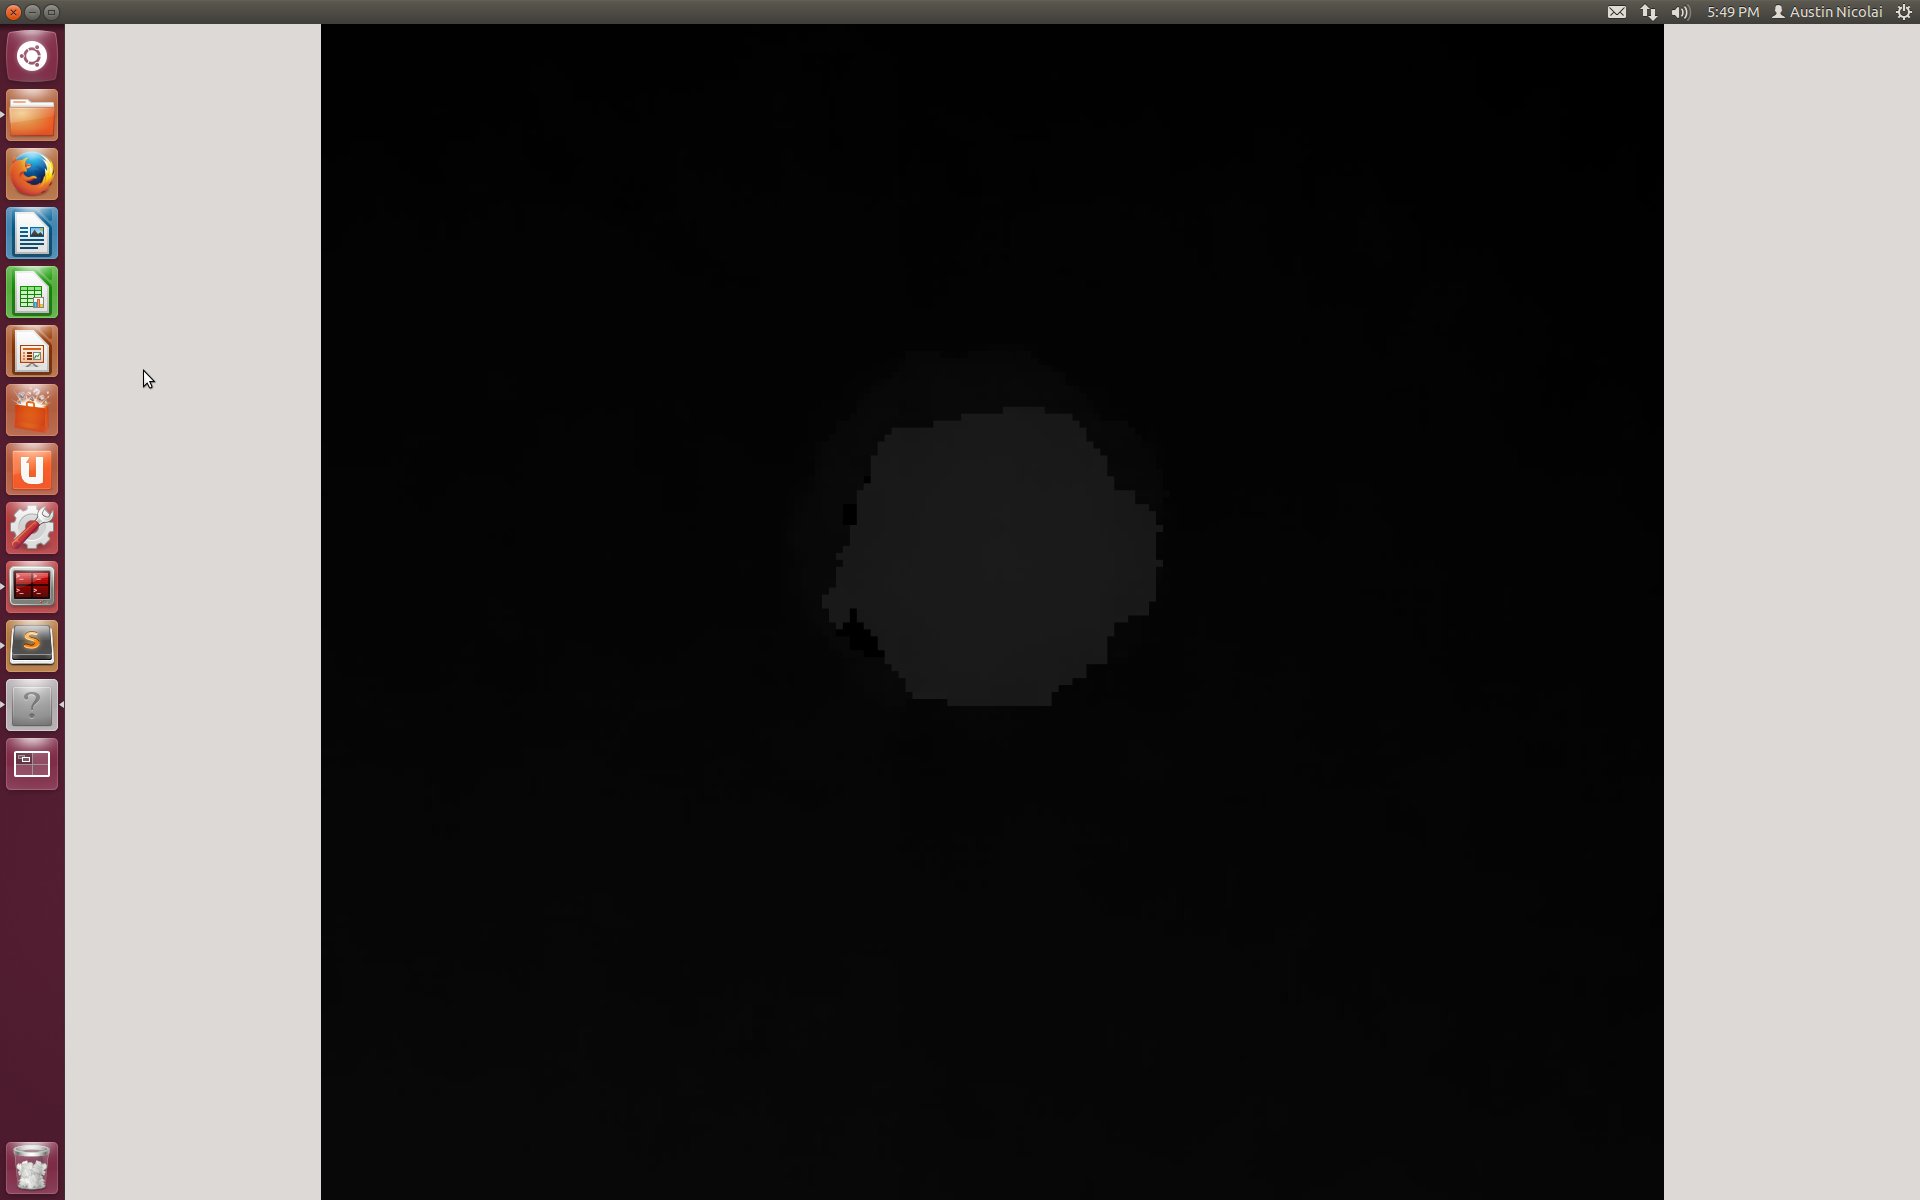
\includegraphics[width=0.3\textwidth]{DH_D_C.png}
    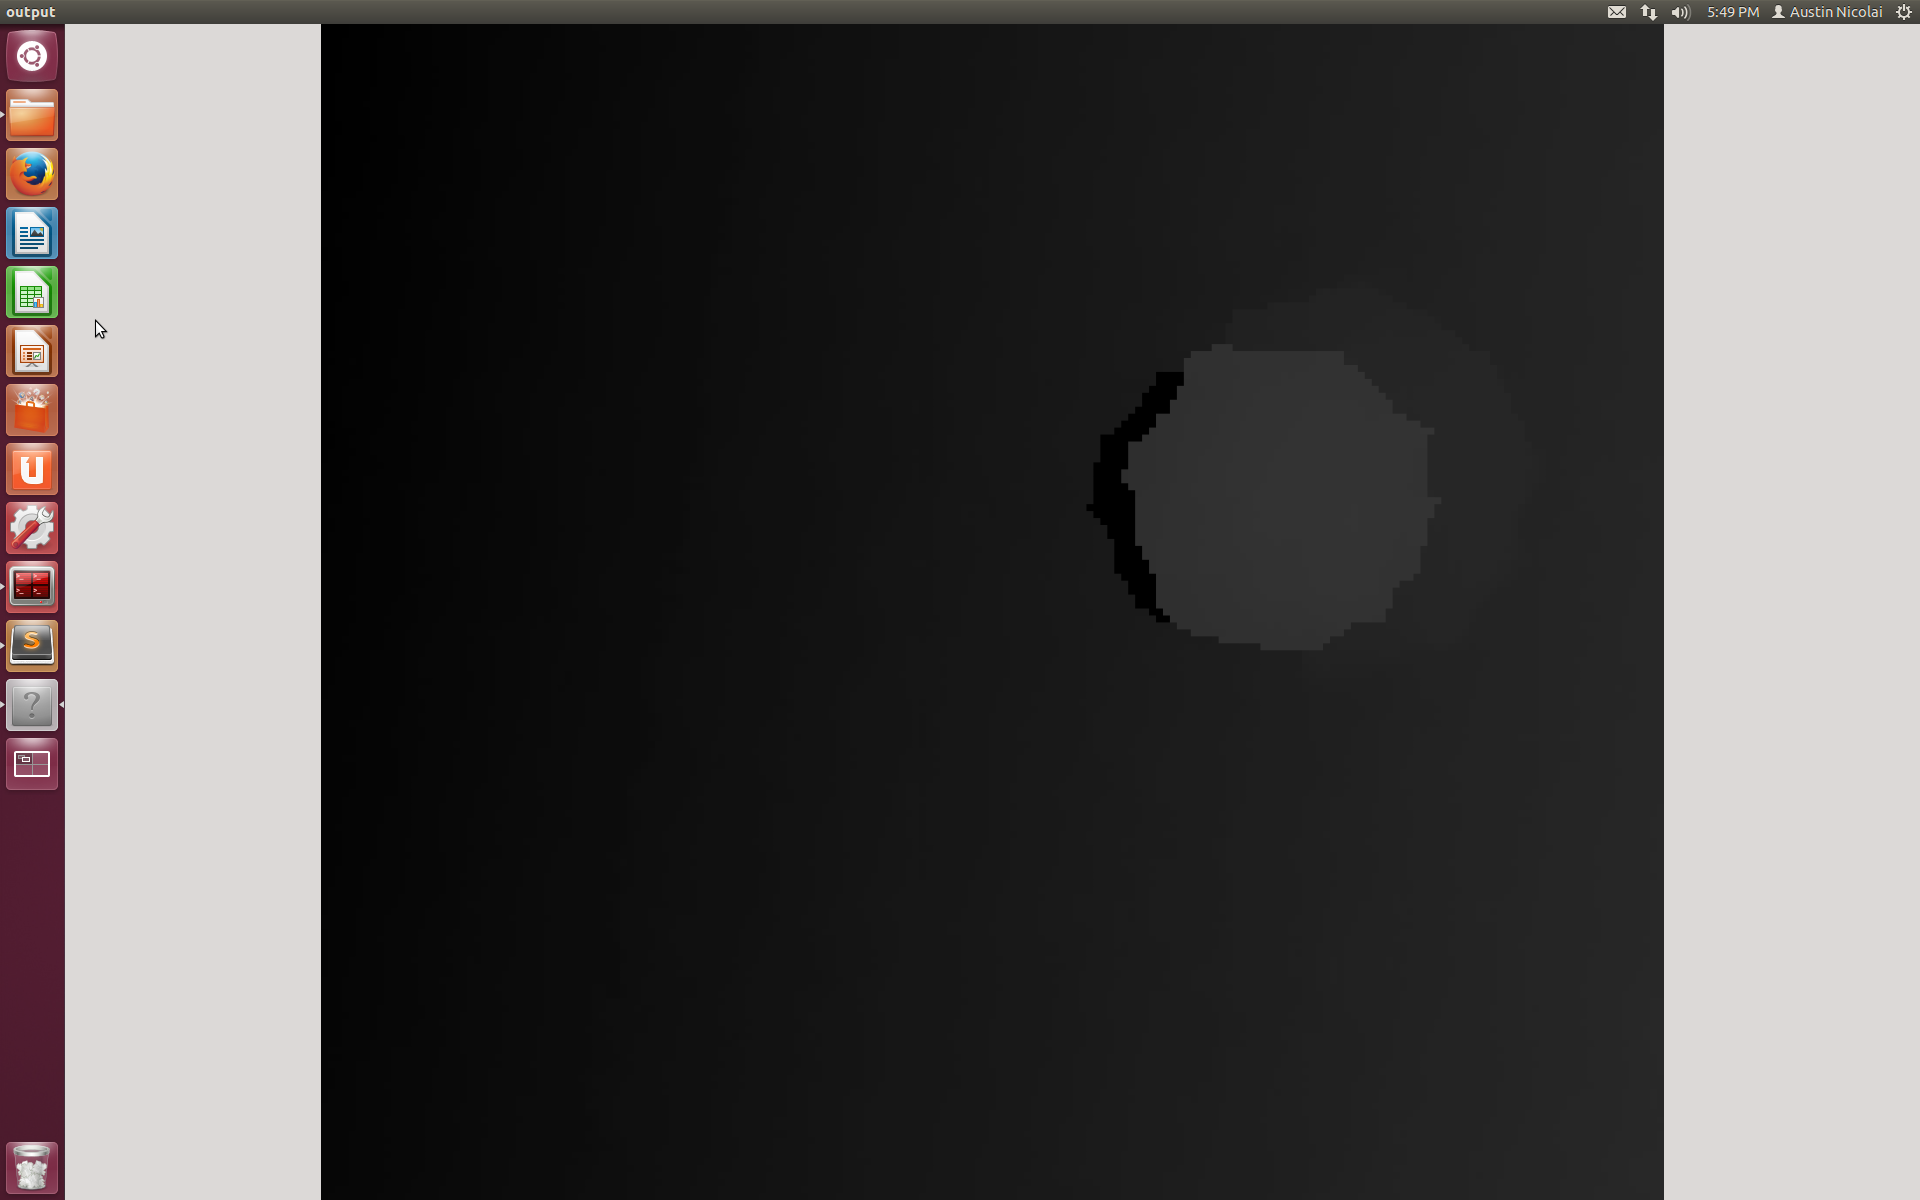
\includegraphics[width=0.3\textwidth]{DH_D_R.png}
    \caption{Door knob data decomposed into the RGB and normalized greyscale depth values as viewed from the left, center and right.}
    \label{fig:decomposition}
\end{figure*}

The depth matrix was then cropped to be a matrix of size 192 x 144 (......Austin....?)

\subsection{Learning}
The data was randomly split into \%80 training data and \%20 testing data. The neural network, which relied upon softmax activation function, consisted of 27,648 inputs, one for each value in the normalized depth matrix.  There were 25 hidden neurons, and 5 outputs. The outputs were the class labels for the 4 knobs plus the blank backdrop.  The neural network was trained using backpropagation for 1000 epochs. Training time lasted approximately 8 hours.

\section{Results}
\begin{figure}[h!]
    \centering
    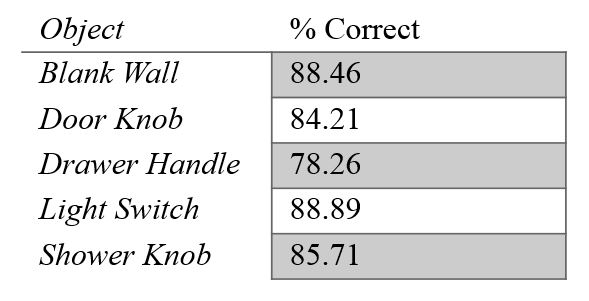
\includegraphics[width=0.6\textwidth]{Results_1.JPG}
    \caption{...explain...}
    \label{fig:results1}
\end{figure}
\begin{figure}[h!]
    \centering
    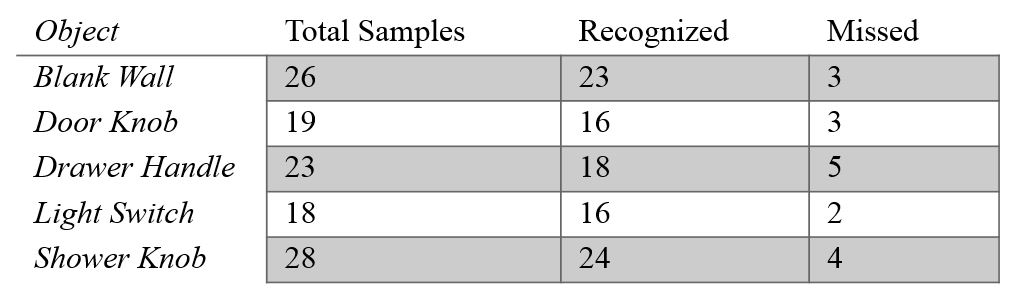
\includegraphics[width=0.9\textwidth]{Results_2.JPG}
    \caption{...explain...}
    \label{fig:results2}
\end{figure}
Overall, classification for the four objects was very high, much greater than random. As can be seen in figure?, if a knob was misclassified, it was classified as a lightswitch. This is probably due to the 

\begin{figure}[h!]
    \centering
    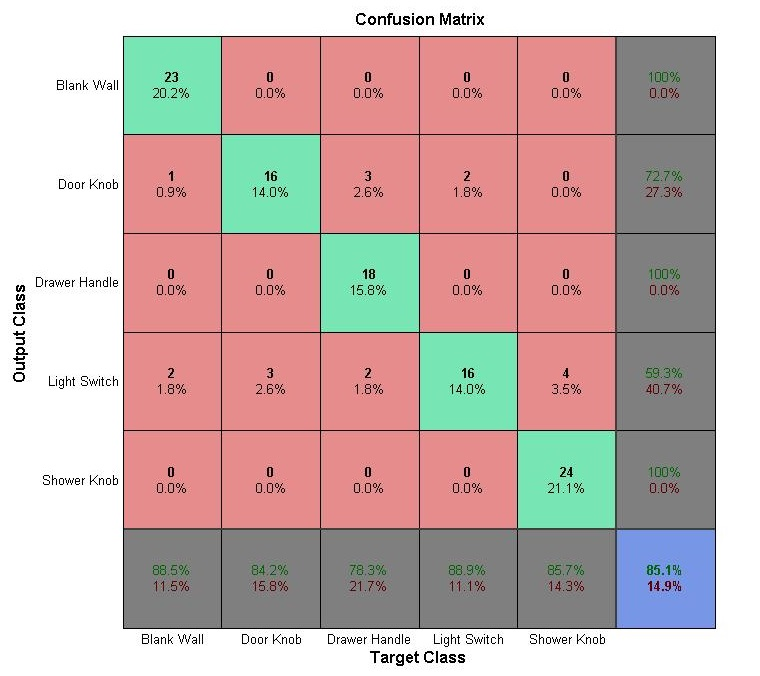
\includegraphics[width=.8\textwidth]{confusion.jpg}
    \caption{Confusion table....explain...}
    \label{fig:confusion}
\end{figure}

Even though the training time on the neural network was longer than we hoped, it was of such duration that the robot could ''train'' on a new set of objects could take place while a person was away at work, or while a person slept.

\section{Future Work}
The analysis of both our domain and results presents several avenues for further research.

-package into ros module
-tie into shared automony interface..
-train on more objects
-pca or some sort of dimension reduction
-try against different learning algorithms

\subsection{Buildit!}
bam!

\bibliographystyle{IEEEtran}
\bibliography{main}


\end{document}
